%% If you have any problems using this template, please contact the author: %%
%% Chris Carmona: carmona@stats.ox.ac.uk ; chriscarmona.me %%

\documentclass{beamer}
\usepackage{tcolorbox}
\usepackage{lipsum}

% fonts
\usepackage[scaled=0.92]{helvet}   % set Helvetica as the sans-serif font
\renewcommand{\rmdefault}{ptm}     % set Times as the default text font

% dmb: not mandatory, but i recommend you use mtpro for math fonts.
% there is a free version called mtprolite.

% \usepackage[amssymbols,subscriptcorrection,slantedGreek,nofontinfo]{mtpro2}

\usepackage[T1]{fontenc}
\usepackage{amsmath}
\usepackage{amsfonts}

% page numbers
\usepackage{fancyhdr}
\fancypagestyle{newstyle}{
\fancyhf{} % clear all header and footer fields
\fancyfoot[R]{\vspace{0.1in} \small \thepage}
\renewcommand{\headrulewidth}{0pt}
\renewcommand{\footrulewidth}{0pt}}
\pagestyle{newstyle}

% geometry of the page
\usepackage[top=1in, bottom=1in, left=1.625in, right=1.625in]{geometry}

% paragraph spacing
\setlength{\parindent}{0pt}
\setlength{\parskip}{2ex plus 0.4ex minus 0.2ex}

% useful packages
\usepackage{natbib}
\usepackage{epsfig}
\usepackage{url}
\usepackage{bm}

%% Information (author, title, etc.) %%


\hyphenation{is-te-ri-nya}

\title[Perbedaan]{% short title for footer
    Perbedaan Anda dan Pasangan Anda: \\
    \textit{A Spiritual Journey}
}

\author{Hendra Bunyamin}

\institute{
%        \textit{Program Studi Teknik Informatika}\\
%        \textit{Universitas Kristen Maranatha}
        \textit{ }\\
		\textit{ }
        \vspace{0.5cm}
}
\date[Venue and Date]{% short date for footer
    31 Januari 2024
}

% ===========================================
%   Added to show ToC before new section
% ===========================================
\AtBeginSection[]
{
	\begin{frame}<beamer>{}
		\tableofcontents[currentsection,currentsection]
	\end{frame}
}

%% Content of slides %%
%%%%%%%%%%%%%%%%%%%%
\begin{document}
%%%%%%%%%%%%%%%%%%%%

% Title slide %
{
    \setbeamertemplate{footline}{}
    \setbeamertemplate{headline}{}
    \setbeamercolor{background canvas}{bg=oxfordblue}
    \maketitle
}

%----------------------------%
% Contents slide
%\setbeamerfont{section in toc}{size=\Large}
%\begin{frame}{}
%%\frametitle{Outline}
%\tableofcontents
%\end{frame}
%----------------------------%

%now include the slides
\setbeamercovered{transparent}
%----------------------------%
%\section{Origin of Marriage}
\begin{frame}{}
	\Large
	\begin{tcolorbox}[colback=green!5,colframe=green!40!black,title=Kejadian 2:18 (TB)]
		TUHAN Allah berfirman: "\textit{\textbf{Tidak baik}, kalau manusia itu seorang diri saja. Aku akan menjadikan penolong baginya, yang sepadan dengan dia.}"
	\end{tcolorbox}
\end{frame}

\begin{frame}{}
	\Large
\begin{tcolorbox}[colback=green!5,colframe=green!40!black,title=Kejadian 1:26 (TB)]
Berfirmanlah Allah: "Baiklah Kita menjadikan manusia menurut gambar dan rupa Kita, supaya mereka berkuasa atas ikan-ikan di laut dan burung-burung di udara dan atas ternak dan atas seluruh bumi dan atas segala binatang melata yang merayap di bumi."
\end{tcolorbox}
\end{frame}

\begin{frame}{}
	\LARGE
	\centering
	\textit{We were designed for relationships}.
	
	\bigskip
	\normalsize
	- \citet{keller2013themeaning}
\end{frame}

\begin{frame}{}
	\LARGE
	\centering
	\textit{Family and relationships are a greater blessing and provide greater satisfaction than anything money can buy}.
	
	\bigskip
	\normalsize
	- \citet{keller2013themeaning}	
\end{frame}

\begin{frame}{}
	\LARGE
	\centering
	\textit{'ezer} = helper-companion, a friend
\end{frame}

\begin{frame}{}
	\Large
\begin{tcolorbox}[colback=green!5,colframe=green!40!black,title=Kejadian 2:23 (TSI)]
Maka laki-laki itu berkata, "Inilah dia yang cocok bagiku! Tulangnya dari tulangku, dan dagingnya dari dagingku! Aku akan menyebut dia 'perempuan', karena dia diambil dariku."
\end{tcolorbox}
\end{frame}

\begin{frame}{}
	\Large
	\begin{tcolorbox}[colback=green!5,colframe=green!40!black,title=Efesus 5:28 (TB)]
		Demikian juga suami harus mengasihi isterinya sama seperti tubuhnya sendiri: Siapa yang mengasihi isterinya mengasihi dirinya sendiri.
	\end{tcolorbox}
\end{frame}

\begin{frame}{}
	\LARGE
\centering
Perkawinan adalah hubungan manusia yang \textbf{paling dasar} dalam kehidupan kita.
\end{frame}



% \section{Spiritual Friendship}
\begin{frame}{}
	\LARGE
	\centering
	Spiritual Friendship
\end{frame}

\begin{frame}{}
	\LARGE
	\centering
	\textit{\textbf{Spiritual Friendship}}:\\ 
	eagerly helping one another know, serve, love, and resemble God in deeper and deeper ways
\end{frame}

\begin{frame}{}
	\Large
	\begin{tcolorbox}[colback=green!5,colframe=green!40!black,title=Efesus 5:25 (NLT)]
		For husbands, this means love your wives, just as Christ loved the church. He gave up his life for her.
	\end{tcolorbox}
\end{frame}

\begin{frame}{}
	\Large
	\begin{tcolorbox}[colback=green!5,colframe=green!40!black,title=Efesus 5:26 (NLT)]
		to make her holy and clean, washed by the cleansing of God's word.
	\end{tcolorbox}
\end{frame}

\begin{frame}{}
	\Large
	\begin{tcolorbox}[colback=green!5,colframe=green!40!black,title=Efesus 5:27 (NLT)]
		He did this to present her to himself as a glorious church without a spot or wrinkle or any other blemish. Instead, she will be holy and without fault.
	\end{tcolorbox}
\end{frame}

\begin{frame}{}
	\LARGE
	\centering
	\textit{You can come as you are, but you CANNOT stay as you are}
	
	\bigskip
	\normalsize
	- Jeffrey Rachmat (JPCC)
\end{frame}


\begin{frame}{}
	\Large
	\begin{tcolorbox}[colback=green!5,colframe=green!40!black,title=Galatia 5:22 (TB)]
		Tetapi buah Roh ialah: kasih, sukacita, damai sejahtera, kesabaran, kemurahan, kebaikan, kesetiaan,
	\end{tcolorbox}
\end{frame}

\begin{frame}{}
	\Large
	\begin{tcolorbox}[colback=green!5,colframe=green!40!black,title=Galatia 5:23 (TB)]
		kelemahlembutan, penguasaan diri. Tidak ada hukum yang menentang hal-hal itu.
	\end{tcolorbox}
\end{frame}

\begin{frame}{}
	\Large
	\begin{tcolorbox}[colback=green!5,colframe=green!40!black,title=Galatia 5:24 (TB)]
		Barangsiapa menjadi milik Kristus Yesus, ia telah menyalibkan daging dengan segala hawa nafsu dan keinginannya.
	\end{tcolorbox}
\end{frame}

\begin{frame}{}
	\Large
	\begin{tcolorbox}[colback=green!5,colframe=green!40!black,title=Galatia 5:25 (TB)]
		Jikalau kita hidup oleh Roh, baiklah hidup kita juga dipimpin oleh Roh
	\end{tcolorbox}
\end{frame}

\begin{frame}{}
	\LARGE
	\centering
	"in-love" experience
\end{frame}

\begin{frame}{}
	\LARGE
	\centering
	1. The Power of Truth
\end{frame}


\begin{frame}{}
	\LARGE
	\centering
	\textit{\textbf{Power of Truth}}:\\ 
	The power to show you the truth about who you are
\end{frame}


\begin{frame}{}
	\LARGE
	\centering
	2. The Power of Love
\end{frame}

\begin{frame}{}
	\LARGE
	\centering
	Marriage puts into your spouse's hand a \textbf{massive power to reprogram} your own self-appreciation
\end{frame}


\begin{frame}{}
	\LARGE
	\centering
	Your heart may condemn you, but \textbf{your spouse's opinion} is greater than your heart
\end{frame}

\begin{frame}{}
	\LARGE
	\centering
	Truth without love ruins the oneness
\end{frame}

\begin{frame}{}
	\LARGE
	\centering
	Love without truth gives the \textbf{illusion of unity} but actually \textbf{stops the journey} and \textbf{the growth}
\end{frame}

\begin{frame}{}
	\LARGE
	\centering
	3. The Power of Grace
\end{frame}

\begin{frame}{}
	\LARGE
	\centering
	\textit{Forgiveness} dan \textit{Repentance}
\end{frame}

\begin{frame}{}
	\centering
	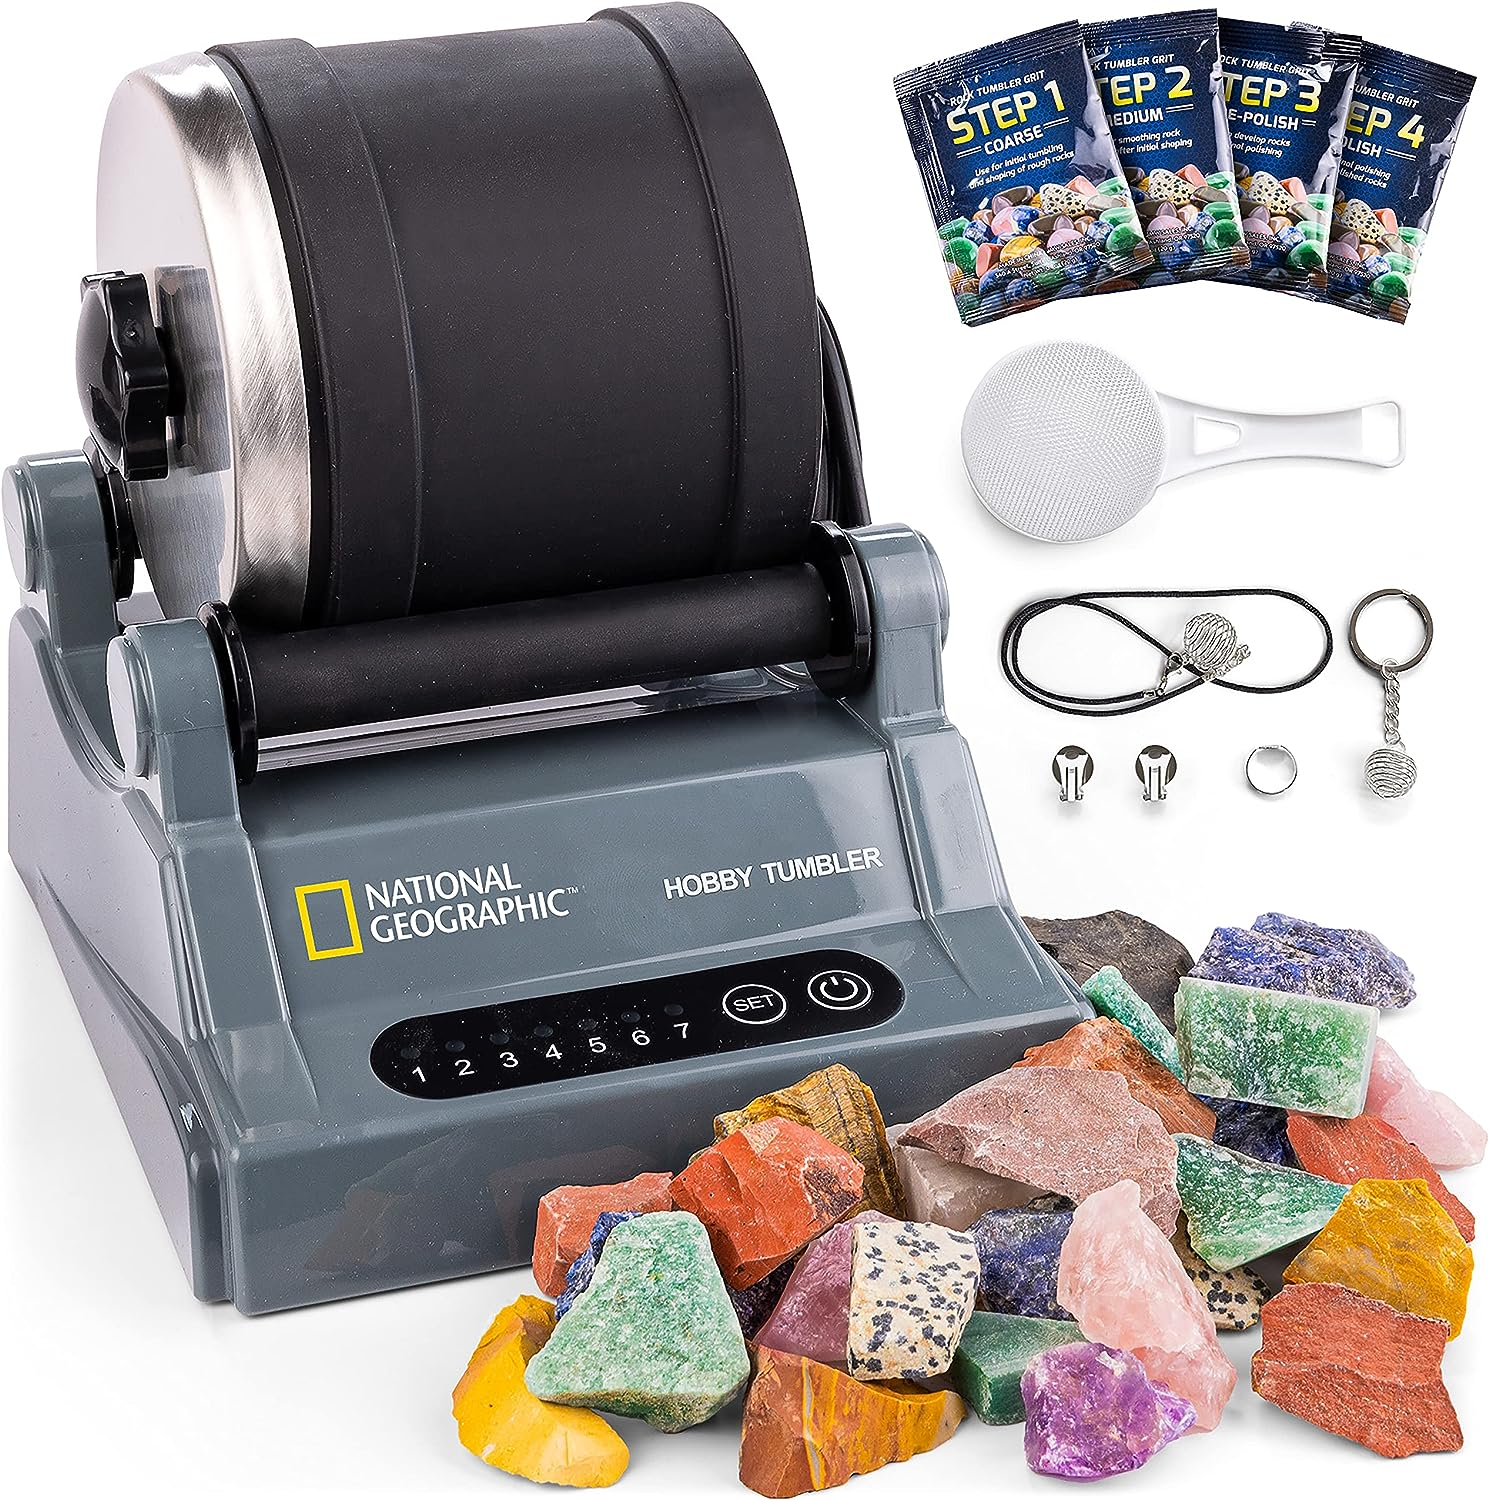
\includegraphics[scale=.15]{images/gem-tumbler-01}
\end{frame}

\begin{frame}{}
	\centering
	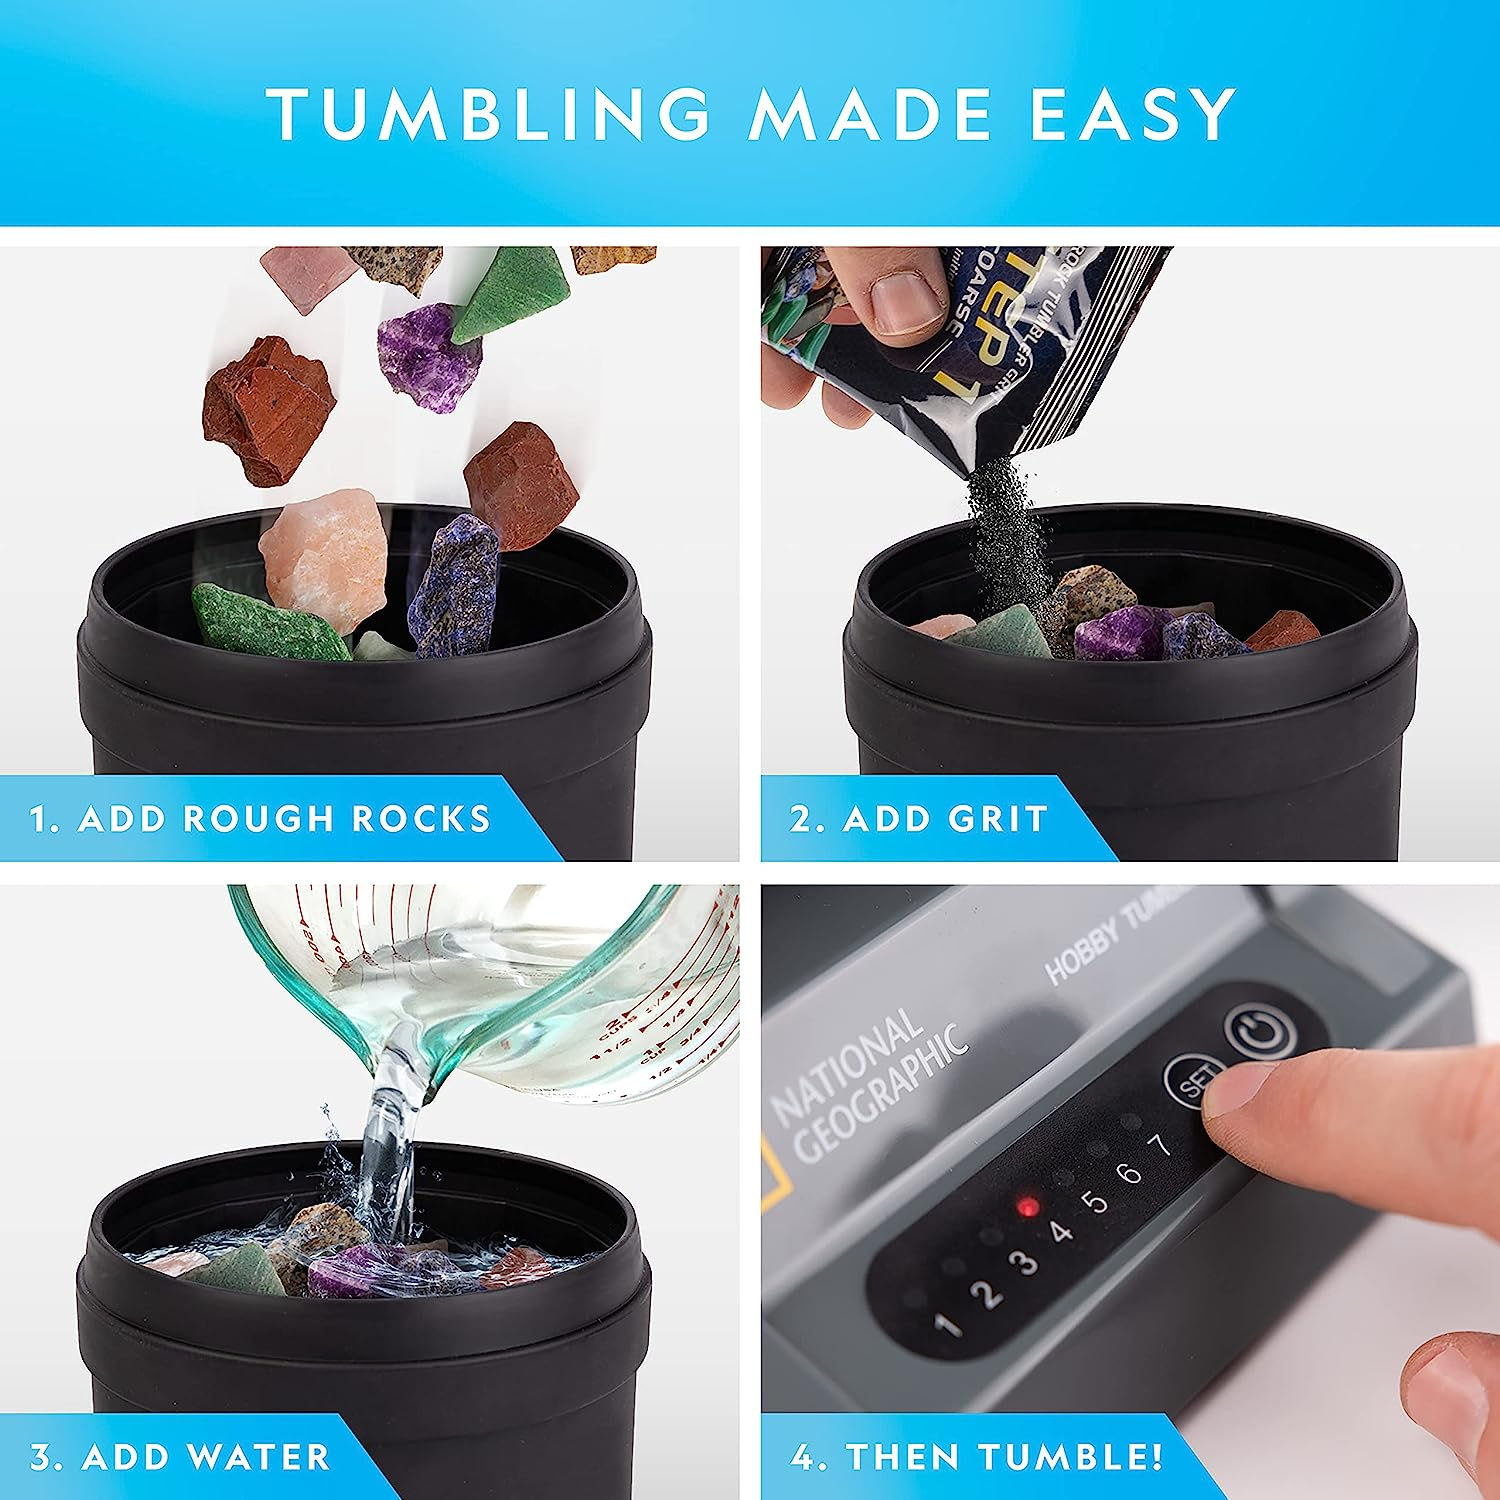
\includegraphics[scale=.15]{images/gem-tumbler-02}
\end{frame}

\begin{frame}{}
	\centering
	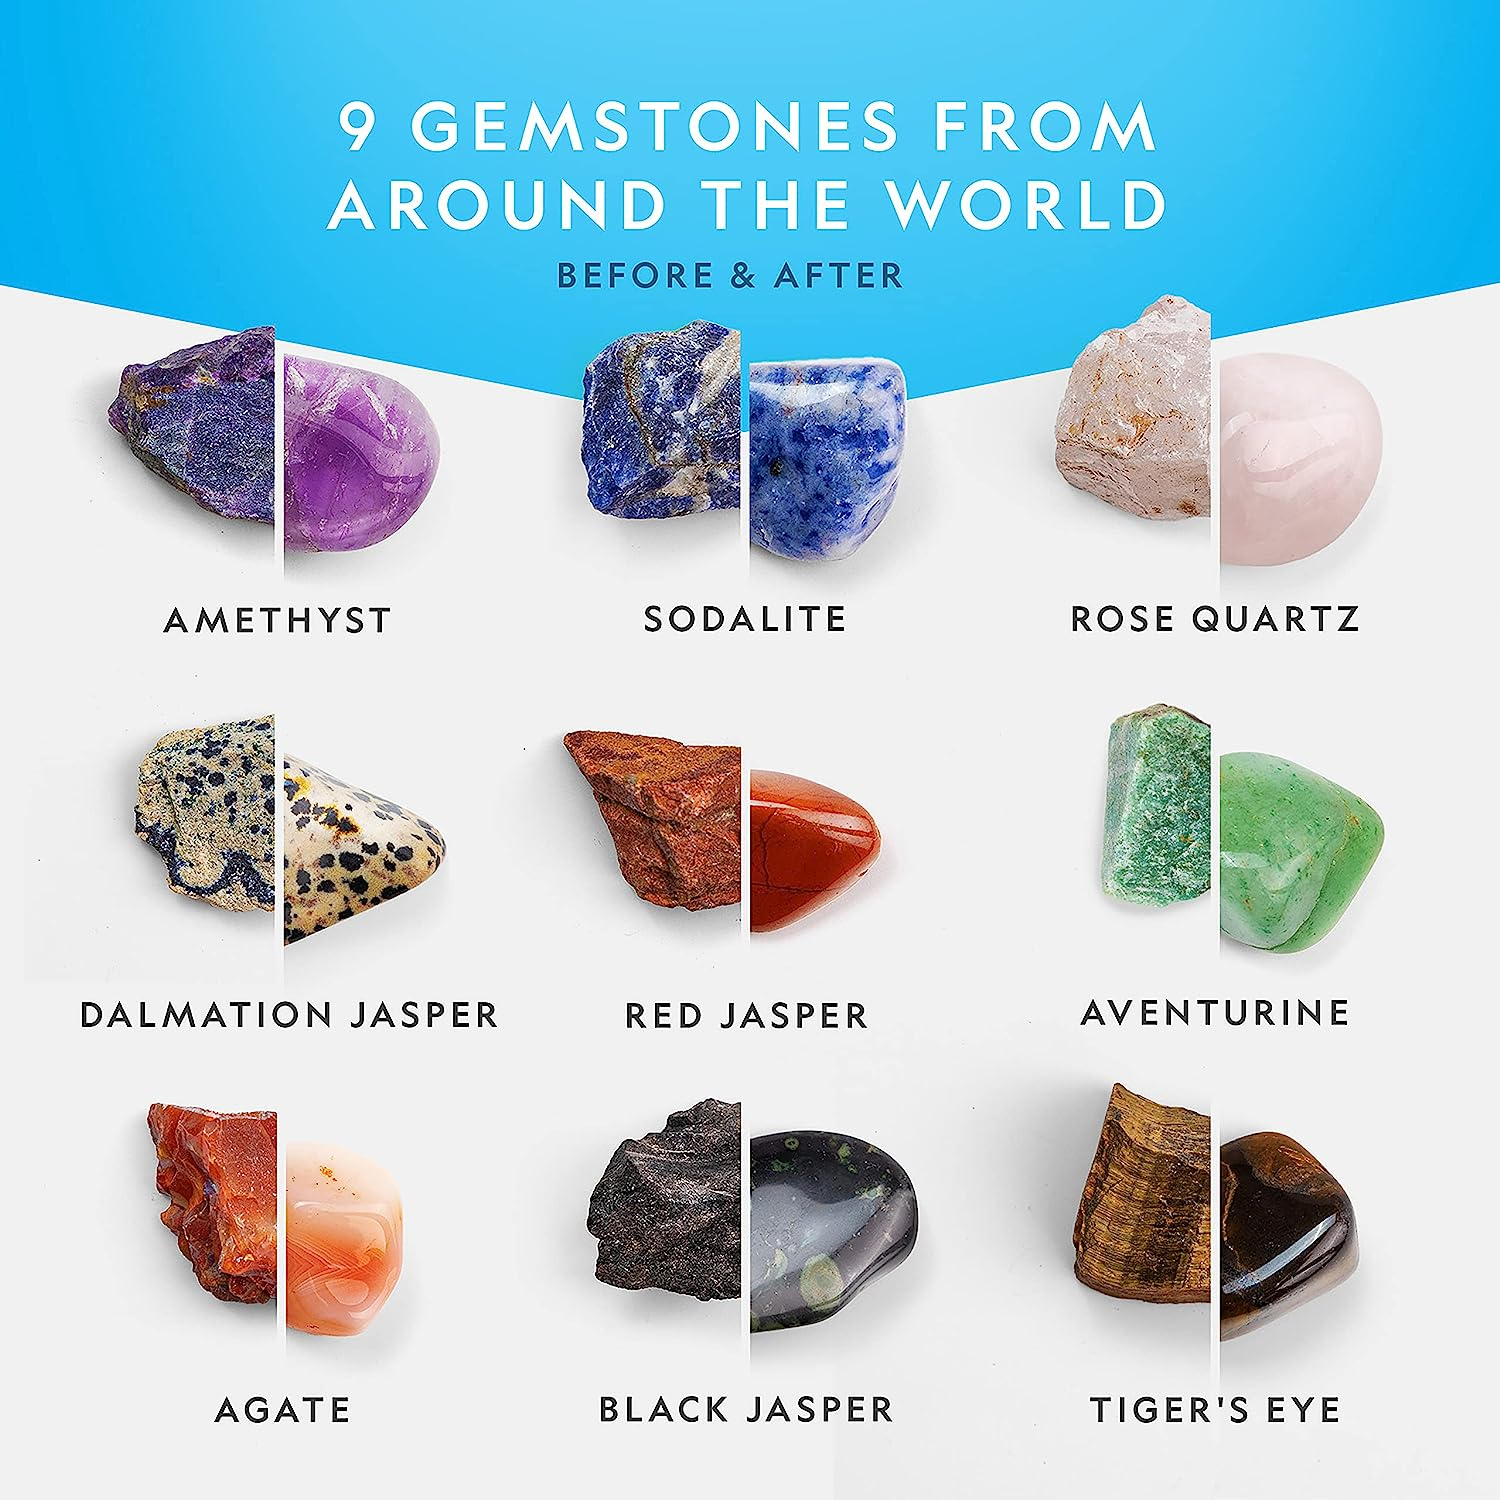
\includegraphics[scale=.15]{images/gem-tumbler-03}
\end{frame}

\begin{frame}{}
	\centering
	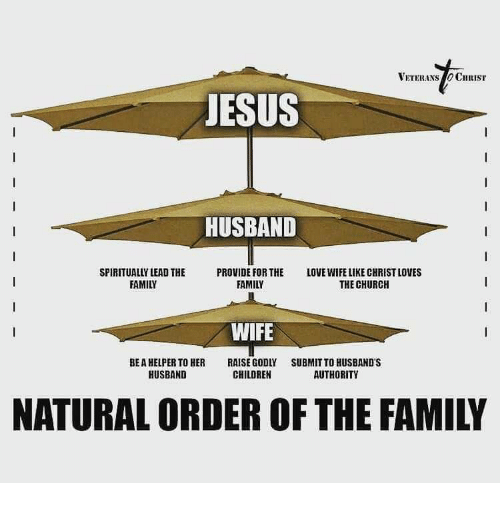
\includegraphics[scale=.475]{images/natural-order-in-a-family}
\end{frame}


\begin{frame}{}
	\Large
	\begin{enumerate}
		\item Sejak anda kenal pasangan anda sampai sekarang, adakah perbedaan yang anda alami bersama pasangan? 
		Coba ceritakan... Bagaimana cara anda mengatasi perbedaan tersebut?
		
		\bigskip
		\item Dari pengalaman anda selama pacaran, pernahkah anda mengalami keributan yang disebabkan oleh perbedaan antara anda dan pasangan? Coba sharing-kan
	\end{enumerate}
\end{frame}	









%----------------------------%



%----------------------------%
% Conclusions
\begin{frame}
    \frametitle{}
    \centering
    
    \huge\color{oxfordblue}
    Terima kasih, \\
    Tuhan Yesus memberkati.

\end{frame}
%----------------------------%

% References slide
\begin{frame}
\frametitle{Daftar Pustaka}
\small
\bibliographystyle{apalike} %use the apalike bibliography style
\bibliography{references} % bibliography file
\end{frame}

%%%%%%%%%%%%%%%%%%%%
\end{document}
%%%%%%%%%%%%%%%%%%%%
